\documentclass{standalone}
\usepackage{tikz}
\usepackage{ctex,siunitx}
\usepackage{tkz-euclide}
\usepackage{amsmath}
\usetikzlibrary{patterns, calc}
\usetikzlibrary {decorations.pathmorphing, decorations.pathreplacing, decorations.shapes,}
\begin{document}
\small
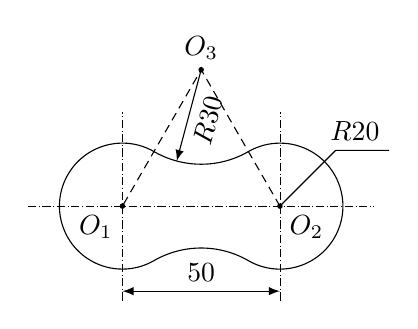
\begin{tikzpicture}[>=latex,scale=0.4]
  \draw([shift=(60:2)]-2.5,0)arc(60:300:2)arc(120:60:3)arc(240:480:2)arc(-60:-120:3);
  \fill([shift=(60:5)]-2.5,0)circle(2.5pt)node[above]{$O_3$};
  \fill(2.5,0)circle(2.5pt)node[below right]{$O_2$};
  \fill(-2.5,0)circle(2.5pt)node[below left]{$O_1$};
  \draw[->]([shift=(60:5)]-2.5,0)--++(-105:3)node[midway,sloped,below]{$R30$};
  \draw(2.5,0)--++(45:2.5)--++(1.7,0)node[above left]{$R20$};
  \draw[densely dashed](2.5,0)--++(120:5)--++(-120:5);
  \draw[very thin,densely dashdotted](-5.5,0)--(5.5,0)(-2.5,-3)--(-2.5,3)(2.5,-3)--(2.5,3);
  \draw[<->](-2.5,-2.7)--(2.5,-2.7)node[midway,above]{50};
\end{tikzpicture}
\end{document}